\documentclass{sigchi}

% Use this command to override the default ACM copyright statement (e.g.
% for preprints). Consult the conference website for the camera-ready
% copyright statement.

%% EXAMPLE BEGIN -- HOW TO OVERRIDE THE DEFAULT COPYRIGHT STRIP -- (July 22, 2013 - Paul Baumann)
% \toappear{Permission to make digital or hard copies of all or part of
% this work for personal or classroom use is 	granted without fee provided
% that copies are not made or distributed for profit or commercial
% advantage and that copies bear this notice and the full citation on the
% first page. Copyrights for components of this work owned by others than
% ACM must be honored. Abstracting with credit is permitted. To copy
% otherwise, or republish, to post on servers or to redistribute to lists,
% requires prior specific permission and/or a fee. Request permissions from
% permissions@acm.org. \\ {\emph{CHI'14}}, April 26--May 1, 2014, Toronto,
% Canada. \\ Copyright \copyright~2014 ACM ISBN/14/04...\$15.00. \\ DOI
% string from ACM form confirmation}
%% EXAMPLE END -- HOW TO OVERRIDE THE DEFAULT COPYRIGHT STRIP -- (July 22, 2013 - Paul Baumann)


% Arabic page numbers for submission. Remove this line to eliminate page
% numbers for the camera ready copy \pagenumbering{arabic}


% Load basic packages
\usepackage{balance}  % to better equalize the last page
\usepackage{graphics} % for EPS, load graphicx instead \usepackage{times}
\usepackage{times}
\usepackage{url}
\usepackage{xspace}

% llt: Define a global style for URLs, rather that the default one
\makeatletter \def\url@leostyle{%
\@ifundefined{selectfont}{\def\UrlFont{\sf}}{\def\UrlFont{\small\bf\ttfamily}}}
\makeatother \urlstyle{leo}




% To make various LaTeX processors do the right thing with page size.
\def\pprw{8.5in} \def\pprh{11in} \special{papersize=\pprw,\pprh}
\setlength{\paperwidth}{\pprw} \setlength{\paperheight}{\pprh}
\setlength{\pdfpagewidth}{\pprw} \setlength{\pdfpageheight}{\pprh}

% Make sure hyperref comes last of your loaded packages, to give it a
% fighting chance of not being over-written, since its job is to redefine
% many LaTeX commands.
\usepackage[pdftex]{hyperref} \hypersetup{ pdftitle={SIGCHI Conference
Proceedings Format}, pdfauthor={LaTeX}, pdfkeywords={SIGCHI, proceedings,
archival format}, bookmarksnumbered, pdfstartview={FitH}, colorlinks,
citecolor=black, filecolor=black, linkcolor=black, urlcolor=black,
breaklinks=true, }

% create a shortcut to typeset table headings
\newcommand\tabhead[1]{\small\textbf{#1}}



\newcommand{\insertpicture}[2]{\begin{center}\includegraphics[width=#2
		\textwidth]{#1}\end{center}}
\newcommand{\etal}{\textit{et al.}\xspace}
\DeclareRobustCommand{\cagatay}{\c{C}a\u{g}atay Demiralp\xspace}
\DeclareRobustCommand{\jeff}{Jeffrey Heer\xspace}

% End of preamble. Here it comes the document.
\begin{document}

\title{The VERP Explorer: A Tool for Exploring Eye Movements of
Visual-Cognitive Tasks Using Recurrence Plots}

\numberofauthors{3} \author{ 
	\alignauthor \cagatay \\
	\affaddr{IBM Research}\\
	\email{cagatay.demiralp@us.ibm.com} 
	\alignauthor Jesse Crimele\\
	\affaddr{Tangible Play, Inc} \\
	\email{jesse@playosmo.com} 
	\alignauthor \jeff \\
	\affaddr{University of Washington}\\ 
	\email{jheer@uw.edu}
	\alignauthor Stuart K. Card \\ 
	\affaddr{Stanford University} \\
	\email{scard@cs.stanford.edu} 
}

\maketitle

\begin{abstract} 
Evaluating the effectiveness of the visual design of an
interface is an important yet challenging problem. In this paper, we
introduce The VERP (Visualization of Eye movements with Recurrence Plots)
Explorer, a visual analysis tool for exploring eye movements during
visual-cognitive tasks. The VERP Explorer couples conventional
visualizations of eye movements with recurrence plots that reveal patterns
of re-visitation over time. We apply the VERP Explorer to the domain
of medical checklist design, analyzing eye movements of doctors searching
for information in checklists under time pressure. We find that the recurrence
plots are characterized square recurrence plot "motifs". At a higher level, we introduce the idea that these square motifs are part of a pattern of "visual micro-foraging" in which the searcher searches for a relevant information patch, then spends effort trying to understand the patch well enough to extract the search question answer, repeating the process as necessary. The analysis also reveals unexpected distractors in the design.
\end{abstract}

\keywords{ Visualization, HCI theory, visual search, eye-movements,
	recurrence plots, motifs, quantified recurrence analysis (QRA), sequential
behavior, time series, information foraging theory, visual micro-foraging.
}

% \category{H.5.m.}{Information Interfaces and Presentation (e.g.
% HCI)}{Miscellaneous}

% See: \url{http://www.acm.org/about/class/1998/} for more information and
% the full list of ACM classifiers and descriptors. \newline
% \textcolor{red}{Optional section to be included in your final version,
% but strongly encouraged. On the submission page only the classifiers’
% letter-number combination will need to be entered.}

\section{Visual-Cognitive Interaction} Cognitive interaction with visual
displays drives many interactive human-computer systems; yet, designing and
engineering such systems can be problematic. General principles can be
applied in generating the display, but it is difficult to  understand the
details of how the principles affect actual user behavior. Adding to the
difficulty, a principle may be right in general, but defeated by
particulars of a given case. Better methods for understanding how well a
visual-cognitive design is working would be helpful. 

Fortunately, eye movements afford a window into sequential visual-cognitive
interactions. But eye movements are at a different behavioral level from
the design decisions being addressed, requiring anecdotal use of
observations or questionable aggregation methods. This paper proposes a set
of analytical methods that may help with this problem, especially the
specific problem of visual search. Our methods have two main goals: (1) to
raise the level of the behavioral characterization for the designer so that
she may more easily understand the good and bad characteristics of a
prototype visual design for a given system, and (2) to package the methods
into an integrated tool, The VERP (Visualization of Eye Movements using
Recurrence Plots) Explorer, so as to make them easy and rapid to use. In
order to accomplish these purposes we characterize the sequential behavior of
eye movements using recurrence plots (rp's), 
motifs (rp patterns), and recurrence quantification analysis (RQA). Our analysis leads us to
the proposal that visual search can be additionally characterized at an even
higher level, by a variety of information foraging theory we term visual
micro-foraging, for which we propose visualizations and micro-foraging
quantification metrics. As an illustration of their use, we apply these
methods to the analysis of designs for emergency medical checklists for
hospital operating rooms.


\begin{figure*}
	\insertpicture{figures/interface.pdf}{0.85}
	\caption{The VERP Explorer interface.\label{fig:interface}}
\end{figure*}

\subsection{Eye Movements} Eye movements afford a window into
visual-cognitive interactions. Eye movements are part of the brain's strategy to trade time-resolution for bandwidth. Spacially, the high bandwidth part of the eye, the fovea, covers only a very small portion, from the center of the visual field out to about 1 deg, of eccentricity.
 In this small region, the eye is densely packed with the cones required for
color vision and high resolution. From about $1\sim 5$ deg, the mixed cones and rods
of the parafovea, provide resolution too low for reading 12 pt text, but enough cones remain for limited color~\cite{Kieras_2014}.  Beyond $ 5$ deg is
the periphery, consisting predominantly of rods that can detect large, high-contrast
features and motion. If we combine the field for the two eyes, the
periphery extends about 130 deg high and 200 deg wide and consists of low spatial
frequency blobs. Neglecting the specialized eye movements for image stabilization and pursuit, dynamically, the small, high-resolution portion of the eye jerks and pauses across  the visual field, assembling an integrated view of the world gleaned during the pauses at a time resolution of about three
samples per second. This implies that there are about 150,000-200,000
eye-movements per day every day for life, requiring that eye-movements be
metabolically very cheap.  The eye is constantly moving, sampling from the
visual field to build up a percept or to attend to areas of high
information content, such as moving objects. The successions of eye
movements extract interpretations from high-information features like sharp
corners and gestalt continuity. As objects are examined, their locations
become visually indexed so that search time to relocate them is reduced. As
a result, objects may form a spatial external working memory indexed
relative to large, low spatial frequency, blobby features. Eye movements
are under competing control of the task, the attraction of unknown
high-contrast blobby elements, and a continuous monitoring for movement or
change. The upshot is that eye-movements tend to track the sequential
attention of the user giving important clues into the detail of
visual-cognitive interaction, but the clues are not always straight-forward
to interpret. 


\subsection{Visualizing Eye Movements} Advances in eye-tracking capability
and practicality has brought increased interest in developing better visual
analysis methods for eye-movement data~\cite{Blascheck_2014}. There are
several standard techniques for visualizing eye-tracking data, including
heat maps, focus maps, and gaze plots (scan paths)~\cite{Holmqvist_2011}. 

Heat map visualizations are widely used for displaying aggregated patterns
of eye movements. However, they suffer from over saturation when the
underlying data is dense.  Heat maps can also be misleading if the color
map isn’t chosen carefully~\cite{Borland_2007}. Related to heat maps are
focus maps.  A focus map is an image mask that shows the underlying
stimulus image at eye-tracking points.  The degree of visibility at a
particular stimulus region is proportional to the density of the tracking
points at that region.  Missing from heat maps and focus maps is a temporal
view of the data. Understanding temporal patterns in eye tracking is
important as they change not only by the visual stimulus but also by the
task~\cite{Yarbus_1967}. Animated heat maps and gaze plots are widely used
to visualize the time ordering in eye tracking data. Animations may,
however, cognitively overload viewers trying to grasp the temporal
context~\cite{TVERSKY_2002}. 

Understanding differences and similarities in eye movements across subjects
is an important goal in eye-tracking studies. However, basic configurations
of heat maps and gaze plots suffer from visual clutter when the underlying
eye tracking data is dense~\cite{Blascheck_2014}. Prior work uses several
techniques to reduce visual clutter and support multi-subject comparisons.
Raschke \etal ~\cite{Raschke_2012} introduce a parallel scan-path
visualization to facilitate the comparison of eye-tracking data across
users.  Earlier research also applies the space-time cube visualization to
eye movement trajectories~\cite{Li_2010,Kurzhals_2013}. Originally proposed
for geographic movement analysis~\cite{Hagerstrand_1970,Kraak_2003}, the
space-time cube visualization treats time as the third—spatial—dimension,
enabling static visualizations of multiple eye-movement trajectories in 3D.
Reducing visual complexity often requires aggregating and sampling the
data, while introducing simpler abstract representations without losing the
original data context.  Burch \etal introduce saccade plots that combine
a heat map  and a graph-based matrix representation for aggregated movement
directions~\cite{Burch_2014b}. Experts often capture semantics of eye
movements by tagging areas of interest (AOIs) on the stimulus image and
associating them with fixations.  This also reduces the cognitive
complexity as the experts care more about what the viewers look at than
where they look at. Prior research borrows from text visualization
techniques to visualize AOIs. Tsang \etal~\cite{Tsang_2010} applies the
WordTree visualization ~\cite{Wattenberg_2008} to AOI tags concatenated
based on their order in eye-movement trajectories. Similar to
ThemeRiver~\cite{Havre_2000}, AOI Rivers~\cite{Burch_2013} visualizes
fixation frequencies of AOIs as flow maps. While the spatial context is
accessible only indirectly, the flow map visualization reduces the visual
clutter that would be otherwise caused by use of gaze plots. The VERP
Explorer couples several of the standard eye-tracking visualizations above,
including heat maps, focus maps, gaze plots, with recurrence plots and
other new visualizations through interaction. 
	
% \pagebreak	

\subsection{Recurrence Plots} 
Recurrence  plots are a type of non-linear
analysis that has been used in the study of dynamical systems and other
areas~\cite{Eckmann_1987,Marwan_2008} In a recurrence plot, some
function is parametrized by time.  For example, Figure~\ref{fig:lorenz} 
shows the Lorentz Function. Notice that it is a multidimensional function
parametrized by time. To obtain the matrix $[r_ij]$ that is the basis for
a recurrence plot, we start with the first eye-position $f_1$  and compare
it to all the other eye-positions in the sequence, including itself. If the
distance  between the two compared eye positions is within some small
distance, as indicated by the two dots in~\ref{fig:lorenz}, then we 
put a 1 at that position in the matrix, otherwise a 0. 

\[ 
r_{ij} = \left\{
	\begin{array}{l l} 
    1  & \quad \text{if $d_{ij} \leq \epsilon$}\\ 
    0  & \quad \text{otherwise} 
    \end{array} \right. 
\]

Coloring all of the one-cells white and the zero-cells white, we get
the recurrence plot in Figure~\ref{fig:lorenz}).

\begin{figure}
	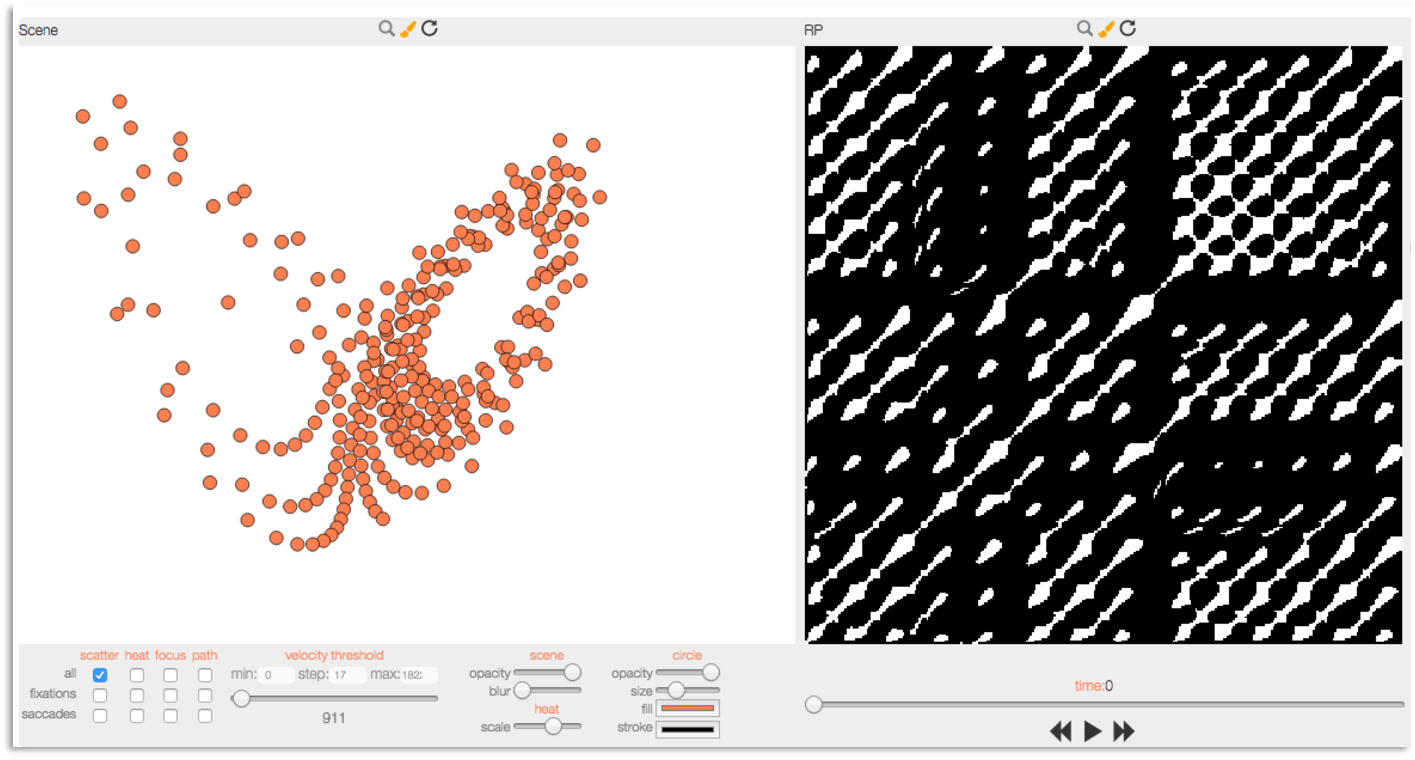
\includegraphics[width=0.23\textwidth]{figures/lorenz.pdf}\qquad
	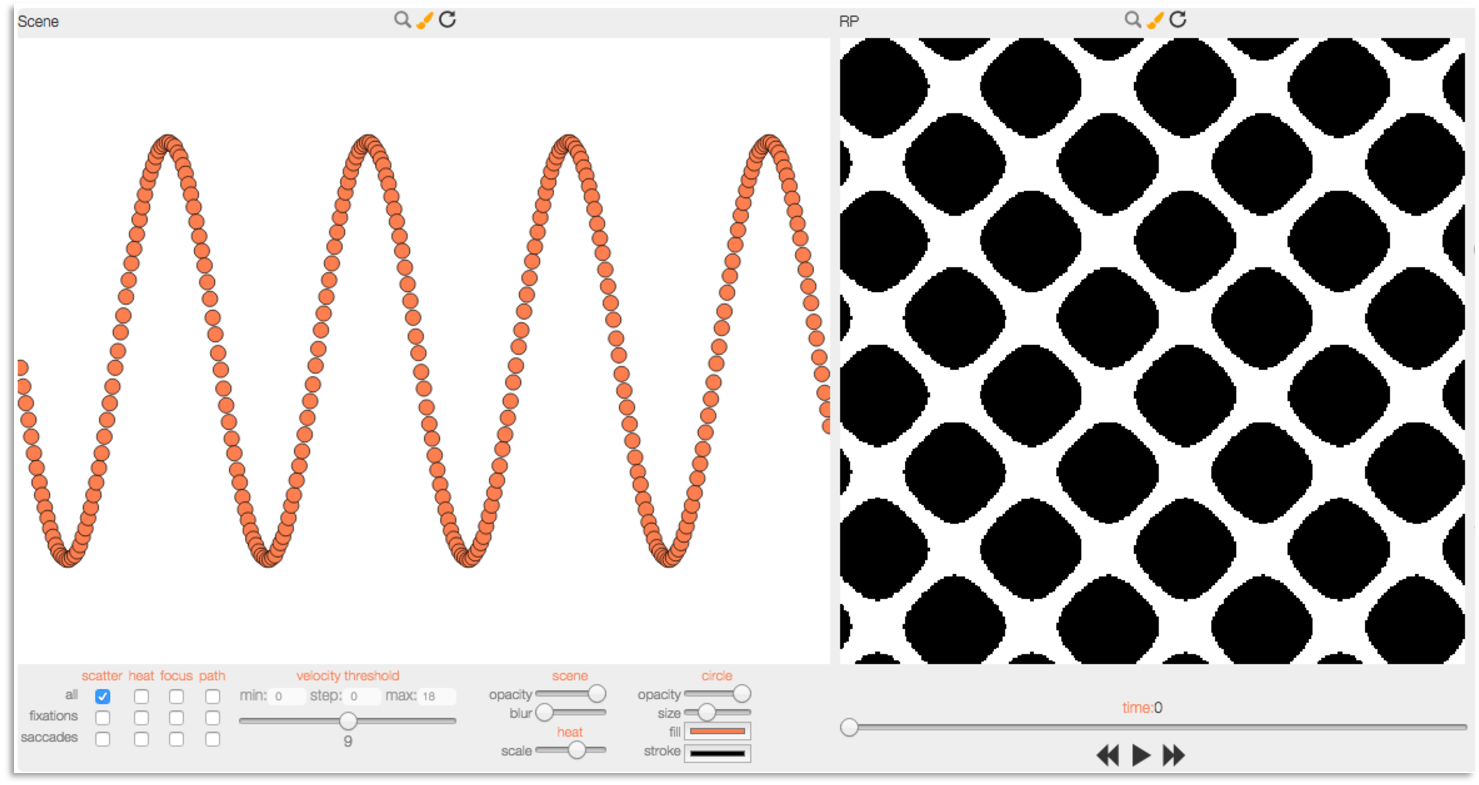
\includegraphics[width=0.23\textwidth]{figures/sine.pdf}
	\caption{Recurrence plot of the Lorenz Function (projected into the
		plane).\label{fig:lorenz}}
\end{figure}


Recurrence plots are particularly good at picking up
periodic and semi-periodic sequences. The recurrence graph of a sine wave
shown on the left of Figure~\ref{fig:sine}, for example, exhibits strong
periodic behavior in the recurrence plot shown on the right. Recently
recurrence plots have recently been applied to eye movements
~\cite{Anderson_2013} for natural scene viewing. In this paper, we integrate previous
techniques of eye-movement and recursion plot analysis into an interactive
tool, simplifying exploratory analysis. We use the tool to study visual
search, which to our knowledge has not been studied in this way. 
We find  a higher level organization for the behavior revealed by 
the eye movements and to propose visualization of this behavior.  


Figure~\ref{fig:construct} shows in more detail how a recurrence graph for eye
movements is constructed. We start with a {\emph scene} Figure~\ref{fig:construct}a
representing  a set of eye-movements plotted over the (static) scene in the
field of view of the participants. The small circle outside of the eye
fixation location indicates the 1 to 2 deg fovea (we shall use 1.5° in our
illustration) around the point of regard. For our purposes, one eye
fixation overlapping the circle of another will be considered as the same
point of regard. That is, $\epsilon = \text{diameter of the fovea} = 2
\times 1.5 deg = 3 deg $. 

\begin{figure}
	\insertpicture{figures/sine.pdf}{0.45}
	\caption{
    Recurrence plot (right) of a sine wave (left).
    \label{fig:sine}
    }
\end{figure}


Given a sequence of eye movements, we draw circles around each fixation
point to indicate the 1.5 deg foveal area in which a person could read the
text. To construct the recurrence plot Figure ~\ref{fig:construct}i of
Figure~\ref{fig:construct}a, we start with a blank matrix Figure~\ref{fig:construct}b whose cells are the width of the foveal area. Eye fixation 1  is within its own
circle so cell (1, 1) is white (Figure~\ref{fig:construct}c). Likewise, 
all other fixations fall within their own circles, so the diagonal (i, j) 
is white (Figure~\ref{fig:construct}d). No other fixations falls within 
the circle of fixation 1, so the rest of row 1 is black 
Figure~\ref{fig:construct}e. 

Since the matrix is symmetric, the rest of column 1 is black as well
(Figure~\ref{fig:construct}f). 

Fixation 2  is also not quite in any other fixation’s circle, therefore,
except for the cell (2, 2) on the diagonal, its row and column are black
(Figure~\ref{fig:construct}g). 

Fixation 3 is in the circle of both fixation 4  and fixation 5, so cells
(3, 4) and (3, 5) are white, by symmetry, so are cells (4, 3) and (5, 3)
(Figure~\ref{fig:construct}h). Finally, fixation 4 is in the circle of fixation,
so (4, 5) and (5, 4) are white (Figure~\ref{fig:construct}i).


\begin{figure}
	\insertpicture{figures/rpconstruction.pdf}{0.45}
	\caption{ Construction of a recurrence plot. \label{fig:construct}}
\end{figure}




\section{Design of The VERP Explorer}
Our primary goals for developing the VERP Explorer were to first to provide
an interactive tool for applying recurrence-based analysis, integrating it
with other eye movement techniques, and second to use these methods to get
a higher order representation of the analyzed behavior, especially in
regard to visual search. Figure~\ref{fig:interface} shows a screenshot 
for the VERP Explorer tool.  In the tool eye movement data are plotted 
twice: in the scene view on the left and in the recurrence plot view on the right.  
Both views are coordinated through brushing and linking. We now discuss the design of
visual representations and interaction techniques in the VERP Explorer to
support these goals. 

\subsection{Heat Maps, Focus Maps, and Scatter Plots} 
The VERP Explorer enables users to visualize eye-tracking positions 
as heat maps, focus maps, and scatter plots. While all the three
methods primarily encode eye-movement positions and are typically 
overlaid on the stimulus scene, they have complementary strengths.  

{\emph Heat maps} and {\emph focus maps}[xx FIX] are two related standard 
visualization techniques that are useful for providing a synaptic view of 
eye movements aggregated over time and subjects. The VERP Explorer creates 
the heat map visualizations by drawing semi-opaque disks centered at 
eye-tracking positions. The disks are filled with a color gradient and 
their opacity is modulated (decreased) with the distance from the disk 
center (Figure~\ref{fig:spatial}). By painting eye-movement point densities, 
heat maps obscure, however, the areas of attention when overlaid on the 
stimulus image. Focus maps visually “invert” heat maps to enable the  
visibility of the areas of viewer attention. To create a focus we  
first create a uniform
image (mask) that has the same size as the underlying stimulus image. We 
then vary the opacity at each pixel inversely proportional to the opacity 
of the corresponding heat map pixel. Focus maps are essentially negative 
space representations, visualizing the negative space of the corresponding 
heat maps (Figure~\ref{fig:spatial}). 

Heat maps and focus maps visualize eye movements indirectly, facilitating
visual aggregation. On the other hand, {\em scatter plots} provide a
discrete view by representing eye-movement positions directly. The VERP
Explorer creates scatter plot views by drawing each eye tracking position
as a circular node in the plane (Figure~\ref{fig:spatial}). Scatter plots 
are useful for
seeing patterns and outliers in eye-movements, while enabling the
inspection of individual eye-movement positions. We also use the scatter
plot view for the timeline animation, as it provides a  discrete
representation of the tracking positions.

\begin{figure*}
	\insertpicture{figures/spatial.pdf}{0.9}
	\caption{ Three spatial eye-tracking visualizations from the VERP
		Explorer: Heat map (left), focus map (middle), and scatter plot
		(right). \label{fig:spatial} }

\end{figure*}

\pagebreak

\subsection{Scan Paths} In their basic, static configuration, neither heat
maps nor focus maps convey the temporal order of eye movements.  The VERP
Explorer uses scan paths (gaze plots) to provide an aggregate temporal view
of eye movements. It creates scan path views by drawing circles centered at
the centroids of fixation clusters and connecting two consecutive clusters
with arrows. The VERP Explorer numbers the nodes sequentially. It also
encodes the temporal order of fixations by coloring the nodes and the
arrows using a color map ranging from dark blue to red~\cite{Harrower_2003}
(Figure~\ref{fig:scanpath}).  We generate the fixation clusters using the velocity-threshold
fixation (I-VT) algorithm~\cite{Salvucci_2000}.  I-VT is a fast and robust
algorithm for identifying fixations and saccades based on their
point-to-point velocities.  I-VT operates under the assumption that
low-velocity eye movements correspond to fixations, while high velocities
to saccade. We now describe the algorithm briefly. See~\cite{Salvucci_2000}
for a detailed, comparative discussion of fixation identification
algorithms. Using I-VT, we compute clusters of fixations in three steps. We
first calculate point-to-point velocities for each tracking point.  Note
that velocities can be computed using spatial or angular distance between
consecutive points.  We use angular velocities if the head position is
provided in the tracking data. We then classify each point as a fixation or
saccade using a velocity threshold (our default value is 300°/s).  If the
point’s velocity is below the threshold, it becomes a fixation point,
otherwise it is considered a saccade points. The VERP Explorer lets users
interactively modify the velocity threshold using a sliding bar. In the
final step, we gather consecutive fixation points into identical clusters
and compute associated measures such as the cluster centroid and duration.
We set the minimum cluster size to twenty. Clusters with fewer than twenty
fixation points are discarded. 

\begin{figure}
\insertpicture{figures/scanpath.pdf}{0.5}
\caption{Scan path.\label{fig:scanpath}}
\end{figure}	

\subsection{Alpha Patches}

Visual clutter is often a concern in eye tracking data visualization.  We
introduce $\alpha$-patches, $\alpha$-shapes~\cite{Edelsbrunner_1994} of 
fixation points, to provide a cleaner view of underlying eye-movement 
locations. $\alpha$-patches enable users to visualize fixated regions 
as filled polygonal patches. Figure~\ref{fig:alphapatch} shows $\alpha$-shapes 
of a point set with  varying $\alpha$ values.

The $\alpha$-shape is a generalization of the convex hull of a point set
~\cite{Edelsbrunner_1994}. The primary advantage of $\alpha$-shapes over 
the convex hull is that $\alpha$-shapes can recover disconnected, non-convex 
spaces with holes. Specifically, for a given real parameter $\alpha \in [0,\infty)$, 
$\alpha$-balls are balls of radius $\alpha$ centered at the points in P.
The $\alpha$ shape of P is then the union of the convex hulls of the
points whose $\alpha$-balls intersect. The VERP Explorer enables users
to automatically create α shapes of eye-movement positions, which we call
$\alpha$-patches.  

We now discuss our algorithm for deriving α patches. Given an eye
tracking point set (e.g., fixations) and an α value, we generate the α
shape for the point set in three steps. First, we create the Delaunay
triangulation of the set.  Note that the boundary of the Delaunay
triangulation is the convex hull of the points in the set. Second, we
extract, from the Delaunay triangulation, the triangles whose vertices
are within the $\alpha$  distance.   The union of the extracted triangles
is known as the $\alpha$-complex of the point set. In the final step, we
determine the boundary of the $\alpha$-complex and draw them as simple
closed polygons. 
	
In our implementation, we create the Delaunay triangulation once and
extract $\alpha$-complexes for varying---user determined---$\alpha$
values as needed.

	\begin{figure}
		\insertpicture{figures/alphapatch.pdf}{0.5}
		\caption{Alpha patches with increasing alpha values from left to
			right. \label{fig:alphapatch}}
	\end{figure}

\pagebreak

\subsection{Interaction Techniques} 
The visualizations we have described are interactive, giving rise 
to a number active exploration techniques: 

\emph{Zooming \& Panning.} The VERP Explorer provides zooming and panning
interactions on all of the visualizations that it generates. Both zooming
and panning are forms of dynamic visual filtering and essential for
exploring dense eye-movement datasets. 

\emph{Brushing \& Linking.} We use brushing \& linking in the VERP Explorer
to coordinate the scatter plot view of the eye-tracking data with the
recurrence plot view. This is the main mechanism that allows users to
inspect recurrence space and spatial eye movements simultaneously. Brushing
over a location on the scene highlights all the corresponding entries in
the recurrence view.  Conversely, brushing on the recurrence plot
highlights corresponding eye movement positions represented as circular
scatter plot nodes.  Brushing regions  can be resized or moved  using mouse
as well as keyboard.

\emph{Dynamic Filtering.} The ability to interactively aggregate, sample
and filter data is key to exploring and untangling complex datasets. The
VERP Explorer enables to users dynamically change the visualization and
analysis parameters. 

\emph{Epsilon Filtering.} Epsilon filtering enables users to explore custom
ranges of epsilon values  for recurrence plots. These changes are also
reflected in measures calculated.  Users can also select different distance
measures. We provide the Euclidean ($L_{2}$ Norm), the city block ($L_{1}$
Norm), the maximum ($L_{\infty}$ Norm) and the minimum of the absolute
differences along data dimensions and the edit distance.  

\emph{Alpha Filtering.} Similar to epsilon filtering, alpha filtering
enables to change how the alpha parameter of the alpha shapes. 

\emph{Dynamic Fixation-Saccade Classification.} The VERP Explorer also
allows users to change the threshold for fixation-saccade classification
dynamically. This is particularly useful when angular velocity calculations
are not possible or reliable. 

\emph{Timeline Animation.} While the scan path visualization provides an
aggregate temporal  view of the  eye movement, it is desirable to be able
to directly examine the timeline of the complete data.  The VERP Explorer
enables users to animate the appearance of eye tracking points in the
scatterplot view. Users can set the speed of the animation or manually
control it by dragging the animation slider’s handle. 

\emph{Motif Search.} Recurrence plots facilitate pattern-based analysis of
time varying data. One of the motivations of the current work is to relate
behavioral eye-movement patterns to visual design through recurrence
patterns. The VERP Explorer enables users to search for predefined patterns
in the recurrence plot. 


\subsection{Recurrence Quantification Analysis} 
There needs to be a method for comparing groups

Developing quantitative metrics expressing features of recurrence plots is one way in which we can compare groups of subjects, trials, tasks, or visual situations and is called Recurrence Quantification Analysis (RQA).  Several measures have been proposed in the general recurrence plot literature. Anderson ~\cite{Anderson_2013} selected a set a set of measures likely to be useful for eye movements. We implemented Anderson's set in VERP. These include:

\emph{Recurrence Rate (RR).} This is the percentage of cells in the
recurrence plot that are white. It measures how many of the visual
positions in the scene are looked at more than once. In general recurrence
plots, this metric is strongly affected by the value chosen for $\epsilon$.
But since we have a natural way of setting epsilon as equal to the foveal
diameter projected onto the display, this metric has more physical meaning.
\[
	RR = {\frac{1}{N(N-1)}}{\sum_{i\neq j}{R(i,j)}}
\]

\emph{Determinism (DET).} This is the proportion of recurrent points
forming diagonal lines. The metric picks up repeated scan patterns.
\[
	DET = 
	\frac{
		\sum_{\ell=\ell_{min}}^{N-1}{\ell H(\ell)}
	}{
		\sum_{i\neq j} { R(i,j) }
	}
\]

\emph{Average Diagonal Line Length (L).} This is meant to pick up the
average length of repeated scan paths.
\[
	L = 
	\frac{
		\sum_{\ell=\ell_{\min} }^{ N-1 }{ \ell H(\ell) }
 	}{
		\sum_{\ell=\ell_{\min} }^{ N-1 }{ H(\ell) }
 	}
\]

\emph{Maximum Diagonal Line Length 
(Lmax)}

\emph{Lmax = xxx}

\emph{Entropy (ENTR).}  Shannon entropy based on diagonal line histograms.
\[
	ENTR = 
    \sum_{\ell = \ell_{\min}}^{N-1}{p(\ell)\ln p(\ell) }
\]
 
\emph{Laminar Phases (LAM).} Analogous to DET, but uses vertical lengths.
\[
	LAM =
	\frac{
		\sum_{v = v_{min} }^{N - 1} { vH(v) }
	}{
		\sum_{i\neq j}{ R(i,j)}
	}
\]
 
\emph{Trapping Time (TT).} Trapping Time is the average length of the
vertical recurrence structures.
\[
	TT = 
	\frac{
		\sum_{v=v_{\min} }^{N-1}{vH(v)}
 	}{
		\sum_{v=v_{\min} }^{N-1}{ H(v)}
 	}
\]

\subsection{Implementation}  The VERP Explorer is a web-based application
and can be accessed at
\url{http://hci.stanford.edu/~cagatay/projects/verp/}. We implemented The
VERP Explorer in JavaScript using D3~\cite{d3_infovis11} and
AngularJS~\cite{angularweb} libraries.  The source code along with example
datasets are also available at \url{https://www.github.com/uwdata/verp/}. 



\section{Illustration of Use: Visual Search in Emergency Medical Checklists}

We now describe a task designed  to serve both as an illustration of the use of the VERP Explorer and a pilot shakedown test as part of VERP's development. As an illustration of the use of the VERP Explorer for exploring a
cognitive-visual task, we will use the task of designing visual displays
for emergency medical checklists. In U.S. hospitals, estimates range in
excess of 100,000 deaths per year associated with preventable harm, and
serious complications may be ten to twenty times more common~\cite{James_2013}. 
In general, these incidents are not caused by lack of skill, but rather by the
complexity of the task.  Checklists have the opportunity for tremendous
impact by helping doctors manage cognitive complexity ~\cite{Gawande_2009}. 
Checklist use improves performance in aviation~\cite{Boorman_2001,Degani_1990,Burian_2005} 
and medicine from  surgery to intensive care and crisis  
response~\cite{Arriaga_2013,Gawande_2009,Harrison_2006, 
Haynes_2009,Makary_2006,Pronovost_2006,Ziewacz_2011}.

However, checklists are not a panacea. Checklists have been criticized for adding
delay, attentional load, and complexity~\cite{Gawande_2009,Winters_2009}, 
slowing down crucial medical procedures. As Verdaasdonk \etal
~\cite{Verdaasdonk_2008}  put it, “Time governs
willingness and compliance in the use of checklists.” 
It would therefore be desirable to improve the speed (and accuracy) 
with which aids can be used.

\subsection{Comparing Two Checklist Formats} For our illustration, we want
to compare two formats for checklists (Figure~\ref{Fig8}). The first format is from the 
World Health Organization and is an example of current best
practice~\cite{James_2013}.  The second is a dynamic format for which 
the current checklist step is enlarged and more distant steps shrunk 
or hidden\cite{Cirimele_2014}.

\begin{figure}

\insertpicture{figures/rqaComparison.pdf}{0.5}
\caption{RQA measures: standard vs. dynamic.\label{fig:rqacomparison}} 

\end{figure}

Participants, who were medical doctors, were seated in a chair at a fixed
distance of approximately 2' from a 22'' monitor with a 1680 × 1050 pixel
resolution. After reading a question, they pressed the spacebar in order to
show the aid. Once they found the answer, they said the answer aloud, and
pressed the spacebar again to advance to the next question. The experiment
measured response time for answers as the interval between spacebar
presses. Each session was videotaped, and a SMI RED eye-tracker captured
participants’ eye movements. This eye-tracker requires no restraint or
equipment to be worn, and is accurate to approximately 0.5 to 1 deg of arc.
For our illustration, we will select only data pertaining to the question:
\emph{What is the correct dose of atropine?} We will only consider data from
five participants and two checklist formats giving us 10 eye-tracker
sessions. Using this illustrative data, we now seek show how The VERP Explorer can help the designer to discover more
insight about the structure of the checklist task and how successful the
proposed design is. 

Figure~\ref{fig:time} shows the comparison between the standard
checklist and our intended improvement. To establish that that the two formats result in different search times, we compute that the average search time for the dynamic format
is 32\% faster than the standard format. Now we use VERP to gain additional insight.  

\emph{Recurrance Plots and Motifs}. VERP outputs from the eye movements of five doctors are
plotted in Figure~\ref{fig10}. They are arranged, within format, in order from the
fastest trials to the slowest trials. The first thing to notice is that the
recurrence plots consist mainly of square patterns with some vertical and horizontal lines. The patterns look nothing like the patterns in Figures [xx fig2] and [xxfig3]. This leads us to our first conclusion. \emph{Eye movements exhibit very different patterns than the semi-periodic function applications investigated in the earlier literature.} We recall the square
pattern from Figure~\ref{fig:construct}. These come about as in Figure~\ref{fig:construct} 
from a group of eye fixation points in close proximity, that is, exhibiting 
locality of reference. The more intensively some part of the scene is exampled, the
larger the size of the square. Some squares have a checkerboard character,
indicating that the doctor shifted her gaze to another part of the scene
and then back .Searches taking more time often  appear more
scattered, reflecting the disorganization of the search. The brushing 
tools provided with VERP allow us to discover where square motifs on 
the recurrence plot are located in the scene. It should be noted that the recurrence plots have been
normalized to the number of eye movements. This means that recurrence plots
to tasks that were accomplished more quickly will have fewer eye movements
and thus the image will appear relatively magnified, exaggerating the
scatter on faster tasks. 

Our second conclusion is that \emph{It would be helpful to formalize more the patterns identified from the recurrence plot and build up catalog of these patterns.}
Recurrence plots often contain
pattern elements that are identifiable building blocks of the recurrence plot and the behavior it expresses. Inspection of the eye movement rp's for our visual search task leads us to here propose the following patterns,  which we will call textual visual search  {\emph motifs}. The patterns we propose are at several levels [xx Fig xx].
At Level 1, the Immediate Level, we are concerned with local patterns that could be detected with a template that looks at a cell and it's immediate neighbors:

\emph{Glance Now—Study Later}. These present as horizontal lines (above the
diagonal). The eyes come back to study something they noted briefly before.

\emph{Study Now—Refer Later}. These present as vertical lines (above the
diagonal). The eyes study something when it is first encountered, then
glance back at it later.

\emph{Study Square.} The dominant motif in the recurrence plot of Figure~\ref{fig:construct} is a study square. It appears in  Figure~\ref{fig:construct} as a consequence of multiple fixation 
points of regard in close proximity. The larger the square, the 
more fixation points, the more intensity is indicated the study.

At Level 2, the Extended Level, we are concerned with how our Level 1 mosaics function as components for a higher level pattern. The Level 2 motifs we have discovered are larger scale versions of the Study Square pattern.

\emph{On-Diagonal Extended Study Square}.  This pattern extends out from the diagonal an indefinite distance. The square indicates a cluster of eye movements in a fixed space, for example trying to extract and act on information on dosage or reading ingredients on a food label.

\emph{Off-Diagonal Extended Study Square}.  Again, the square indicates a cluster of eye movements in a fixed space, for example trying to extract and act on information on dosage or reading ingredients on a food label. These motifs are likely to indicate a distraction or a difficult search.

But the most interesting level of motif we have seen is at Level 3, which we have called the Narration Level. Level 3 is high enough that the patterns relate to the terms of the task.  So
far, we have been considering eye movements individually, but the square
motif in our recurrence plots suggests that they interact in groups: a
sequence of saccades to a position on the checklist followed by a set of
fixations around that area (see [xx Fig FF]) Notice that the square motif
appears regardless of the order of the fixation within the cluster. This
pattern is similar to the patterns found in information foraging
theory~\cite{Pirolli_1999}. 
\begin{figure}
\insertpicture{figures/time2.pdf}{0.4}
\caption{Standard vs. improved times.\label{fig:time}}
\end{figure}

\begin{figure}
\insertpicture{figures/motifs2.pdf}{0.5}
\caption{Motifs.\label{fig:motifs}}
\end{figure}

But the most interesting level of motif we have seen is at Level 3, which we have called the Narration Level. Level 3 is high enough that the patterns relate to the terms of the task.  So
far, we have been considering eye movements individually, but the square
motif in our recurrence plots suggests that they interact in groups: a
sequence of saccades to a position on the checklist followed by a set of
fixations around that area (see [xx Fig FF]) Notice that the square motif
appears regardless of the order of the fixation within the cluster. This
pattern is similar to the patterns found in information foraging
theory~\cite{Pirolli_1999}. 

\subsection{Visual Micro-Foraging} 

According to information foraging theory, the organism is trying to 
maximize the rate of information gain, $R$, which is equal to 
the ratio of net information gain, $U$,  divided by the time spent $T$ in 
foraging.
\[
R  =  \frac{U}
{
T
}
 =  \frac{U_f - \left(C_s + C_h\right)}
{
	T_s + T_h 
	} 
\]

 In the model, the net information gain $U$  is obtained  by    
 subtracting the cost of foraging search, $C_f$,  and handling, $C_h$,  from  
 the total foraging information gain, $U_f$. Similarly, the time spent in 
 foraging is equal to the total time spent  in searching, $T_s$,  and 
 handling, $T_h$. 


\begin{figure*}
	\insertpicture{figures/dummy.eps}{0.8}
	\caption{table of figures \label{fig10}}
\end{figure*}

The pattern can readily be seen in Figure~\ref{fig11}a. The first panel 
shows a set of saccades to find a promising patch (search costs,  $T_s$, which is then intensively studied 
Figure~\ref{fig11}b with fixations to extract the 
needed information (handling costs, $T_h$,).  This approach transforms the way we 
look at the data. The scene can be treated as consisting of information patches. The search
costs are the saccades to find the patch, $T_s$. Handling costs $C_h$ are the costs
associated with actually reading and understanding the information.
Information Foraging Theory suggests two ways to improve the efficiency of
acquiring knowledge from the checklists~\cite{Pirolli_1999}: between-patch enrichment
and within-patch enrichment. Between-patch enrichment means improving the
search to make the desired information easier to find. This has been done
in the case of the Dynamic checklist format by dynamically hiding or
minimizing items not immediate to the currently relevant item in the
checklist and using the space to make the relevant item larger.
Within-patch enrichment means making the desired information easier to
assimilate. An example in the Dynamic format, drug dosage information
follows a rigid format to make it faster to extract the currently need
information. Chernov’s Marginal Utility Theorem~\cite{Stephens_1986)} says 
[Fig Chernov] that whether we do between or within patch enrichment, that the 
time the information searcher spends in a patch should be shortened. 

\begin{figure}
	\insertpicture{figures/dummy.eps}{0.5}
	\caption{Fig Chernov\label{fig:chernov}} 
\end{figure} 

We can use VERP to identify patches automatically. First, we separate search saccades from fixations using the angular velocity threshold of 300 degrees/sec. We then collapse consecutive  fixations into clusters (\ref{section:scanpath}). Each 
fixation cluster  forms  a patch and we number   the patches from 0 
(the starting position of the eye) upwards. To show the searches, we 
draw a line following the saccades.

From[xx  Fig 10?] it is evident
that the smaller information patches, whose construction we have just
described, are part of larger patches. To depict these [xx develop], we use
heat maps. The effect of this analysis is to generate an automatically
generated micro-narrative in pictures of what the participant paid attention to. 


\subsection{Verbal Micro-Narratives} 
We can
go even further with this idea by noting the words under the heat map. For
the fastest trial of the Standard checklist format in [xx fig10?], the words show what the graphic
shows: the participant quickly located the concept, the sets of words in a
patch are similar. The participant quickly found the patch and spent most
of her time trying to understand the content. 

\begin{enumerate}
	\item \ldots Airway (accesses and\ldots  \\
		\ldots Breathing (100\% Get transcutaneous\ldots  \\
		\ldots Atropine (1.5\ldots  
	\item	\ldots for help\ldots  \\
	\ldots transcutaneous pacer\ldots  \\
	\ldots atropine (1.5 ms IV; may\ldots  \\
	\item  \ldots transcutaneous pacer\ldots  \\
		\ldots atropine (1.5 ms IV; may\ldots  \\
    \ldots stimulation if laparoscopy\ldots 
\end{enumerate}

On the other hand, for the slowest time (Fig 10), each set of words in a
patch is quite different, because the participant is lost in the search
part. The sequence of concepts to which the participant responds 
and the visual representation of the sequence of information patches 
searched form a micro-narrative at a behavioral level  above the 
eye movement and recurrence plot levels. This enables us to  quickly 
characterize the participant’s behavior. 
% Dynamic format. 
[replace these with focus visualizations. Xx I was just waiting for those.]

% On the other hand, for the worst time (Fig 10), each set of words in a
% patch is quite different, because the participant is lost in the search
% part. The sequence of concepts to which the participant respond and the
% visual representation of the sequence of information patches searched forms
% a micro-narrative at a behavioral level above the eye movement and
% recurrence plot level that allows the engineer of this system to more
% quickly characterize the participant’s behavior. Dynamic format. 
\begin{enumerate}
	\item \ldots Calcium channel\ldots  \\
		\ldots -Calcium chloride\ldots  \\ 
	  
	\item \ldots Increase the milliamperes\ldots \\

	\item \ldots Consider expert consultation\ldots  
	\item  \ldots Airway (accesses and\ldots  \\
		\ldots Breathing (100\% \ldots \\
	\item	\ldots Beta blocker overdo\ldots  \\
		\ldots Overdose\ldots 
	\item  \ldots Give Atropine\ldots 

\end{enumerate}
\subsection{Gremlins} 
We have concentrated on the general patterns in the eye movements,
but since the eyes are controlled both in reaction to visual
stimuli as well as cognitively in service of a goal, we also
discover unexpected effects--we call them gremlins. Such was the case with these
analyses. In four out of five of the Dynamic format screen shots
in Figure~\ref{fig10}, the eye has been attracted to the pictures of doctors
attending. This features was included in the format, because it
is often the case that attending medical personnel do not know
each other’s names, which in turn makes it difficult to address
direct requests to a named individual—an important element of
disciplined coordination to prevent requesting participant from
thinking some task has been done, whereas no one actually
accepted responsibility for doing it. It did not occur to the
designers of this format that the high contrast of the picture to
the dark background would interfere with the acquisition of
information in the checklist, although this is particular gremlin becomes obvious and visible  once it is
pointed out. Thus the displays of VERP can be useful for pointing
out issues that no-one thought to ask. In general, the Dynamic
format was the better compared format of the two and so tested as in Figure~\ref{fig:time}. But 
this general success masked a gremlin within the design.

\begin{figure}
	\insertpicture{figures/dummy.eps}{0.5}
	\caption{Fig 12\label{fig12}}
\end{figure}


					
\section{Conclusion} 
Evaluating the effectiveness of the visual design of an
interface is an important yet challenging problem. The analysis of eye movements has been recognized as an important technique for this problem, but eye movements are usually at a lower level then the behavior the designer needs to analyze, and eye movements are
This paper proposes a set
of analytical methods that may help with this problem, especially the
specific problem of visual search. Our methods have two main goals: (1) to
raise the level of the behavioral characterization for the designer so that
she may more easily understand the good and bad characteristics of a
prototype visual design for a given system, and (2) to package the methods
into an integrated tool, The VERP (Visualization of Eye Movements using
Recurrence Plots) Explorer, so as to make them easy and rapid to use. In
order to accomplish these purposes we characterize the sequential behavior of
eye movements using recurrence plots (rp's), 
motifs (rp patterns), and recurrence quantification analysis (RQA). Our analysis leads us to
the proposal that visual search can be additionally characterized at an even
higher level, by a variety of information foraging theory we term visual
micro-foraging, for which we propose visualizations and micro-foraging
quantification metrics. As an illustration of their use, we apply these
methods to the analysis of designs for emergency medical checklists for
hospital operating rooms.


\subsection{Visual Search Narrative Analysis}


[***  It is important that you write for the SIGCHI audience.  Please read
previous years' Proceedings to understand the writing style and conventions
that successful authors have used.  It is particularly important that you
state clearly what you have done, not merely what you plan to do, and
explain how your work is different from previously published work, i.e.,
what is the unique contribution that your work makes to the field?  Please
consider what the reader will learn from your submission, and how they will
find your work useful.  If you write with these questions in mind, your
work is more likely to be successful, both in being accepted into the
Conference, and in influencing the work of our field. ***]

\section{Acknowledgments}

xxxxxxxxxxx TODO xxxxxxxxxxxxx
1. Add Pirolli's book to Info foraging refs
2. Make simplified foraging fig tofix current one
3. Fix foraging equaation
4. Cut chernov fig to save space?

% \balance

\pagebreak

\bibliographystyle{acm-sigchi} 

\bibliography{verp} 

\end{document}
